\documentclass[conference]{IEEEtran}

\usepackage{cite}
\usepackage{amsmath,amssymb,amsfonts}
\usepackage{amsthm}
\usepackage{algorithm}
\usepackage{algorithmic}
\usepackage{graphicx}
\usepackage{booktabs}
\usepackage{multirow}

% Theorem environments for the methodology guarantee.
\theoremstyle{plain}
\newtheorem{theorem}{Theorem}
\newtheorem{corollary}{Corollary}
\theoremstyle{definition}
\newtheorem{assumption}{Assumption}
\newtheorem{definition}{Definition}
\theoremstyle{remark}
\newtheorem{remark}{Remark}

\begin{document}

\title{Controlled Machine Unlearning in Continual Learning Via Parameter-Efficient Overlap-Aware Adapters}

\maketitle

\begin{abstract}
Selective forgetting (or machine unlearning) in Continual Learning (CL) architectures aims to intentionally eradicate specific task or domain knowledge from a previously trained deep neural network. The critical constraint of this process is preserving the model's classification fidelity on the remaining active tasks. Conventional unlearning mechanisms, including the standard Privacy-Aware Lifelong Learning (PALL) framework, often suffer from catastrophic degradation due to implicit parameter overlaps between the targeted forgetting datasets and the retention tracking datasets, leading to massive parameter update footprints.

In this paper, we propose two novel, overlap-aware frameworks to mitigate this fundamental trade-off: \textbf{PALL-Modified} and \textbf{PALL-Adapter}. Our first method, PALL-Modified, explicitly computes the critical parameter intersection to prevent overlap degradation, achieving highly competitive retention accuracy via a regularized optimization objective. To address the inherent computational burden of full-network tuning, our second method, PALL-Adapter, replaces full-network gradient tuning with a sub-network modular task adapter architecture coupled with a dynamically regulated shared bottleneck adapter. By confining unlearning updates strictly to specific sub-modular pathways through a novel three-phase soft-masked optimization process (and explicitly unlearning the associated classifier heads), the PALL-Adapter substantially reduces updates to the frozen backbone.

Extensive empirical evaluations across CIFAR-10, CIFAR-100, and TinyImageNet benchmarks demonstrate the robust scalability of our dual-architecture approach. While PALL-Modified yields the highest retention accuracy among the compared methods, PALL-Adapter curtails the requisite updated parameter ratio by up to 87\% compared to full-network variants. Simultaneously, PALL-Adapter limits the maximum performance drop on retained tasks (WorstDrop) to below 1\% in our evaluated multi-task CL settings, providing an effective balance between parameter efficiency and unlearning fidelity.
\end{abstract}

\begin{IEEEkeywords}
Continual Learning, Machine Unlearning, Selective Forgetting, Parameter-Efficient Adapters, Critical Overlap
\end{IEEEkeywords}

\section{Introduction}

The ubiquitous deployment of Deep Neural Networks (DNNs) in real-world, privacy-sensitive applications is increasingly governed by strict legal and ethical data frameworks, most notably the European Union's General Data Protection Regulation (GDPR) \cite{gdpr2016} and the California Consumer Privacy Act (CCPA) \cite{ccpa2018}. These legislative milestones enforce the "Right to be Forgotten" \cite{gdpr2016}, granting individual users the authority to request the deletion of their personal data from trained machine learning systems. Concurrently, modern artificial intelligence relies heavily on Continual Learning (CL) environments, wherein models autonomously and sequentially assimilate knowledge from non-stationary streaming datasets.

While classical CL methodologies focus extensively on mitigating "catastrophic forgetting" \cite{mccloskey1989catastrophic, kirkpatrick2017overcoming}, the emerging problem of selective forgetting (or machine unlearning) introduces an inverse challenge \cite{cao2015towards, bourtoule2021machine}. It necessitates the intentional, surgical removal of specific previously acquired knowledge without inducing catastrophic degradation on the remaining, active tasks.

The dominant barrier to effective selective forgetting within multi-task neural networks is the "parameter overlap" phenomenon. High-capacity neural networks implicitly distribute conceptual representations across vast, entangled arrays of shared parameters. When traditional unlearning techniques, such as unconstrained gradient ascent or Fisher-based network scrubbing \cite{golatkar2020forgetting}, are executed on a target task dataset \(D_f\), they inadvertently disrupt the functional representations of the retained tasks \(D_r\) that rely on those identical parameter spaces.

The original Privacy-Aware Lifelong Learning (PALL) framework \cite{ozdenizci2025pall} was introduced as a mechanism to modularize task knowledge. However, the standard implementation (PALL-Original) still operates over large network sub-spaces and lacks a granular mechanism to control feature-level overlaps, updating on the order of roughly $1$--$4\%$ of a deep network's total parameters per unlearning request \cite{ozdenizci2025pall}.

\textbf{Contributions:} To circumvent these limitations, we propose two distinct, synergistic methodologies:
\begin{enumerate}
    \item \textbf{PALL-Modified:} A mathematically robust extension that explicitly quantifies the "Critical Overlap" between forgotten and active parameters, executing unlearning via a constrained regularization penalty.
    \item \textbf{PALL-Adapter:} A parameter-efficient CL unlearning architecture that freezes the deep feature extraction backbone and reroutes sequential task learning through localized Task-Specific Bottleneck Adapters and a Shared Bottleneck Adapter.
    \item \textbf{Three-Phase Soft-Protection:} We formulate an optimization masking algorithm (Eradication, Quantification, and Soft-Scaling) that explicitly governs gradient updates during unlearning, ensuring that critical shared features remain insulated, while also incorporating an explicit classifier unlearning pathway.
\end{enumerate}

\section{Related Work}

\subsection{Continual Learning and Memory Replay}
The continual learning paradigm seeks to accumulate knowledge across sequentially presented tasks \cite{thrun1995lifelong}. Regularization methodologies, such as Elastic Weight Consolidation (EWC) \cite{kirkpatrick2017overcoming} and Learning without Forgetting (LwF) \cite{li2017learning}, aim to anchor parameters. Experience Replay (ER) and Dark Experience Replay (DER++) \cite{buzzega2020dark} maintain an episodic memory buffer of historical samples. Recently, frameworks such as Continual Learning and Private Unlearning (CLPU) \cite{liu2022clpu} have combined DER++ with task-specific temporary networks, but they often require complex sub-model management.

\subsection{Machine Unlearning Strategies}
Exact unlearning frameworks, such as SISA \cite{bourtoule2021machine}, partition data streams into isolated ensemble models. Approximate unlearning techniques manipulate gradients to scrub information \cite{golatkar2020forgetting}. Boundary Unlearning approaches attempt to shift the decision boundaries of the output space, achieving rapid forgetting speeds \cite{chen2023boundary}. In CL settings, however, unconstrained gradient updates blindly destroy the feature spaces utilized by other active tasks. Saliency Unlearning (SalUn) \cite{fan2024salun} utilizes gradient-based weight saliency to restrict unlearning updates strictly to highly influential weights. Similarly, Selective Synaptic Dampening (SSD) \cite{foster2024ssd} dampens specific parameters proportionally to their Fisher-based importance.

\subsection{Parameter-Efficient Fine-Tuning (PEFT)}
PEFT methods, initially conceptualized in Natural Language Processing via Adapter modules \cite{houlsby2019parameter} and LoRA \cite{hu2021lora}, limit trainable parameters by injecting low-rank bottleneck layers into frozen networks. In CL and unlearning contexts, frameworks like BID-LoRA \cite{rachapudi2026bidlora} and UnCLe \cite{adhikari2026uncle} have demonstrated that PEFT can effectively compartmentalize task knowledge. Our proposed PALL-Adapter framework explicitly maps overlapping representations within these modules to prevent degradation.

\section{Methodology}

\subsection{The Limitation of Unconstrained Forgetting}
In the standard PALL framework, the unlearning process identifies task-specific parameters but fails to dynamically isolate features critical to other active tasks. Consequently, executing gradient ascent on a target task blindly overwrites overlapping decision boundaries, causing catastrophic performance drops (WorstDrop) across retained tasks. Our methodology directly addresses this by explicitly mapping and protecting the functional intersection.

\subsection{Proposed Method 1: PALL-Modified Framework}
To identify critical knowledge boundaries without the full computational overhead of Fisher Information Matrices, we approximate parameter importance using absolute gradients computed over a limited episodic memory (Replay Buffer). Let \(S_{forget}\) represent the top-\(K\) specific subset of parameters exhibiting high gradient sensitivity (\(|\nabla_w \mathcal{L}|\)) to the target data \(D_{forget}\). Let \(S_{active}\) denote the top-\(K\) union of critical parameters necessary to maintain the empirical risk bounds of all actively retained tasks. We explicitly calculate the critical shared intersection:
\begin{equation}
S_{share\_crit} = S_{forget} \cap S_{active}
\end{equation}

Computing \(S_{forget}\) assumes momentary access, at the time of the unlearning request, to a small sample of the target task's own data in order to localize its parameter footprint via \(|\nabla_w \mathcal{L}|\). In our implementation this sample is drawn from the rehearsal buffer and is purged immediately afterward, together with the task's stored exemplars, as part of the same forgetting operation. The privacy cost is therefore bounded: the to-be-forgotten data is touched only to estimate importance and is deleted in situ, leaving no retained copy of the forgotten task.

Rather than optimizing a single combined objective, PALL-Modified separates \emph{forgetting} from \emph{retention repair} into two distinct stages. \textbf{(i) Forgetting (reset).} The weights that are exclusive to the target task---those in its subnetwork but outside the retained-task support, \(S_{forget}\setminus S_{active}\)---are reset to their initialization, erasing the task-specific pathway without any gradient step. \textbf{(ii) Retention repair.} The model is then briefly fine-tuned on the rehearsal buffer of the \emph{remaining} tasks to restore knowledge transfer, minimizing a combined dark-experience-replay and cross-entropy objective with an \(\ell_2\) anchor applied \emph{only} on the critical shared region:
\begin{equation}
\mathcal{L}_{repair} = \alpha\,\mathcal{L}_{DER} + \beta\,\mathcal{L}_{CE} + \lambda \sum_{w \in S_{share\_crit}} \left\| w - w_{old} \right\|^2 .
\end{equation}
Here \(\mathcal{L}_{DER}\) matches the stored logits and \(\mathcal{L}_{CE}\) the labels of the retained tasks, while the final term holds the shared critical weights near their pre-forget values \(w_{old}\). The two stages thus play complementary roles: the reset performs the erasure, and the anchored repair protects the shared functional space, yielding the highest retention accuracy albeit operating over the entire network capacity.

\begin{figure}[t]
    \centering
    \includegraphics[width=\columnwidth]{architecture.pdf}
    \caption{The proposed PALL-Adapter architecture. The backbone is strictly frozen ($\theta_{base}$), while representations are routed sequentially through the Shared and Task-specific Bottleneck Adapters.}
    \label{fig:architecture}
\end{figure}

\subsection{Proposed Method 2: PALL-Adapter Architecture}
To radically reduce the computational overhead and isolate task interference, we freeze the deep feature extraction layers of the primary architecture (\(\theta_{base}\)). The trainable domain \(\Phi\) is constrained solely to:
\begin{enumerate}
    \item \textbf{Shared Bottleneck Adapter (\(\phi_{shared}\))}
    \item \textbf{Task-Specific Adapters (\(\phi_{t}\))}
    \item \textbf{Task-Specific Classifier Heads}
\end{enumerate}

For an input activation tensor \(x\), the forward propagation logic through a residual block utilizing ReLU \cite{nair2010relu} is formulated as:
\begin{equation}
z_{shared} = x + \mathbf{W}_{up}^{(s)} \cdot \text{ReLU}\left(\mathbf{W}_{down}^{(s)} \cdot x\right)
\end{equation}
\begin{equation}
z_{final} = z_{shared} + \mathbf{W}_{up}^{(t)} \cdot \text{ReLU}\left(\mathbf{W}_{down}^{(t)} \cdot z_{shared}\right)
\end{equation}

\subsection{Three-Phase Soft-Masked Unlearning}
The unlearning execution in the PALL-Adapter framework operates through three distinct mathematical phases, explicitly incorporating classifier management:

\textbf{Phase 1: Domain-Specific Eradication.} Without requiring backpropagation, the task-specific module for the forgotten task (\(\phi_{t_{forget}}\)) is instantly destroyed. We reinitialize \(\mathbf{W}_{down}\) via Kaiming distribution \cite{he2015delving} and zero-out \(\mathbf{W}_{up}\), eradicating isolated knowledge pathways. Additionally, the classifier head corresponding to the targeted task is reinitialized to ensure no residual decision boundaries persist.

\textbf{Phase 2: Shared Overlap Quantification.} Utilizing a limited replay buffer, we compute absolute gradients (\(|\nabla \mathcal{L}|\)) strictly over the parameters of the shared adapter \(\phi_{shared}\). This explicitly yields the critical shared overlap \(S_{share\_crit}\) between the target task and retained tasks.

\textbf{Phase 3: Soft-Masked Optimization.} We optimize \(\phi_{shared}\) using standard Cross-Entropy \cite{goodfellow2016deep} to force the target outputs toward a uniform distribution:
\begin{equation}
\mathcal{L}_{unlearn} = \mathbb{E}_{(x,y) \in D_{forget}} \left[ -\sum_{c} \frac{1}{|C|} \log p(y=c|x; \Phi) \right]
\end{equation}
Crucially, gradient updates are dynamically constrained using a \textit{soft-scaling} multiplier (\(m_{soft}\)):
\begin{equation}
\label{eq:softupdate}
w^{(i+1)} = w^{(i)} - \eta \cdot m_{soft}(w) \cdot \nabla_{w} \mathcal{L}_{unlearn}
\end{equation}
Where \(m_{soft}(w)\) is defined as:
\begin{equation}
\label{eq:softmask}
m_{soft}(w) = \begin{cases}
(1.0 - \text{protect\_strength}), & \text{if } w \in S_{share\_crit} \\
1.0, & \text{if } w \in S_{forget} \setminus S_{active} \\
0.0, & \text{otherwise}
\end{cases}
\end{equation}
This mechanism acts as a robust friction barrier, severely dampening updates in the critical overlap region while permitting surgical eradication of exclusively targeted weights.

\begin{figure}[t]
    \centering
    \includegraphics[width=\columnwidth]{overlap_concept.pdf}
    \caption{Conceptual representation of parameter overlap (\(S_{share\_crit}\)). The soft-scaling mechanism acts as a shield over this specific intersection.}
    \label{fig:overlap_concept}
\end{figure}

\subsection{Theoretical Guarantee: Soft-Scaling Bounds the WorstDrop}
\label{subsec:theory}

We now establish that the soft-scaling multiplier of
Eq.~\eqref{eq:softmask} is not a heuristic damping term but a
quantity that provably \emph{contracts} the catastrophic-forgetting
error (the WorstDrop) induced on the active tasks, relative to
standard unconstrained unlearning. Throughout this analysis the deep
backbone $\theta_{base}$ and the task-specific adapters
$\{\phi_{t}\}$ are frozen during the unlearning request; the only
parameters that are mutated, and hence the only parameters capable of
inducing cross-task interference, are the shared bottleneck adapter
weights $\phi_{shared}\in\mathbb{R}^{d}$. We therefore restrict the
entire analysis to $\phi \triangleq \phi_{shared}$.

\subsubsection*{Notation and parameter partition}

Let $\phi^{(0)}$ denote the shared-adapter parameters immediately
before Phase~3 and let $\phi^{(N)}$ denote the parameters after $N$
soft-masked optimization steps. For each coordinate
$i\in\{1,\dots,d\}$ the update of Eq.~\eqref{eq:softupdate} reads
\begin{equation}
\label{eq:coord-update}
\phi^{(k+1)}_{i} \;=\; \phi^{(k)}_{i}
       \;-\; \eta\, m_{i}\, g^{(k)}_{i},
\qquad
g^{(k)}_{i}\;\triangleq\;\partial_{i}\,\mathcal{L}_{\text{unlearn}}\!\left(\phi^{(k)}\right),
\end{equation}
where $m_{i}\in[0,1]$ is the per-coordinate soft-scaling multiplier,
held fixed across the $N$ steps because the masks
$S_{forget},S_{active}$ are computed once in Phase~2. Following the
implementation, the index set $\{1,\dots,d\}$ is partitioned into four
disjoint regions:
\begin{equation}
\label{eq:partition}
\begin{aligned}
\mathcal{F}^{\!\circ} &\triangleq S_{forget}\setminus S_{active}
   && (m_i = 1), \\
\mathcal{S} &\triangleq \big(S_{share\_crit}\big)\setminus H
   && (m_i = 1-p), \\
H &\subseteq S_{share\_crit}
   && (m_i = 0,\ \text{hard-protected}), \\
\mathcal{N} &\triangleq \{1,\dots,d\}\setminus S_{forget}
   && (m_i = 0),
\end{aligned}
\end{equation}
where $S_{share\_crit}=S_{forget}\cap S_{active}$,
$p\triangleq\texttt{protect\_strength}\in[0,1]$ is the protection
strength, and $H$ is the optional hard-protected subset selected
inside the critical overlap (with $H=\varnothing$ recovering the pure
three-case mask of Eq.~\eqref{eq:softmask}).

\begin{definition}[Retained risk and parameter drop]
\label{def:drop}
For an active task $t\in\mathcal{T}_{active}$ let
$R_{t}(\phi)\triangleq\mathbb{E}_{(x,y)\sim D_{t}}\big[\ell\big(f(x;\phi),y\big)\big]$
be its expected risk as a function of the shared adapter. The
\emph{drop} inflicted on task $t$ by an unlearning trajectory
$\phi^{(0)}\!\to\!\phi^{(N)}$ is
$\Delta_{t}\triangleq R_{t}(\phi^{(N)})-R_{t}(\phi^{(0)})$, and the
worst-case interference is
$\mathrm{WorstDrop}\triangleq\max_{t\in\mathcal{T}_{active}}\Delta_{t}$.
\end{definition}

\noindent
The empirical metric of Eq.~\eqref{eq:worstdrop} reports an
\emph{accuracy} drop; Assumption~\ref{ass:lipschitz-acc} below makes
the standard bridge to the risk drop of Definition~\ref{def:drop}
explicit, so that a bound on the risk drop transfers to the reported
quantity up to a fixed constant.

\subsubsection*{Assumptions}

\begin{assumption}[Smoothness of retained risks]
\label{ass:smooth}
Each retained risk $R_{t}$ is $\beta$-smooth on the trajectory's
convex hull, i.e.
$\big\|\nabla R_{t}(\phi)-\nabla R_{t}(\phi')\big\|_{2}\le\beta\,\|\phi-\phi'\|_{2}$.
\end{assumption}

\begin{assumption}[Bounded unlearning gradients]
\label{ass:bounded}
The per-coordinate unlearning gradients are uniformly bounded along
the trajectory, $|g^{(k)}_{i}|\le G$ for all $i,k$, so that the total
coordinate displacement obeys
$\Gamma_{i}\triangleq\big|\sum_{k=0}^{N-1} g^{(k)}_{i}\big|\le NG$.
\end{assumption}

\begin{assumption}[Overlap concentration of retained sensitivity]
\label{ass:concentration}
The sensitivity of every retained task to the \emph{forget-exclusive}
weights is uniformly small: there exists $\epsilon\ge 0$ such that
$|\partial_{i} R_{t}(\phi^{(0)})|\le\epsilon$ for all
$i\in\mathcal{F}^{\!\circ}=S_{forget}\setminus S_{active}$ and all
$t\in\mathcal{T}_{active}$.
\end{assumption}

\begin{assumption}[Accuracy--risk Lipschitzness]
\label{ass:lipschitz-acc}
There is a constant $L_{a}\ge 0$ such that the per-task accuracy drop
is dominated by the risk drop,
$A_{t}^{\text{before}}-A_{t}^{\text{after}}\le L_{a}\,\Delta_{t}$,
for every $t\in\mathcal{T}_{active}$.
\end{assumption}

\noindent
Assumption~\ref{ass:concentration} is precisely the property that
Phase~2 \emph{constructs}: $S_{active}$ is defined as the top-$K$
support of the retained-task gradient magnitude, so any coordinate
that is \emph{not} in $S_{active}$ carries, by definition, a
retained-task gradient below the selection threshold $\epsilon$. The
analysis below is therefore self-consistent with the algorithm rather
than an external regularity condition.

\subsubsection*{Main result}

\begin{theorem}[Soft-scaling contracts the WorstDrop]
\label{thm:worstdrop}
Let Assumptions~\ref{ass:smooth}--\ref{ass:lipschitz-acc} hold and fix
a learning rate $\eta>0$ and step count $N$. Define, for each active
task $t$, the \emph{critical interference energy}
\begin{equation}
\label{eq:Ecrit}
E^{\mathrm{crit}}_{t}\;\triangleq\;
\eta\!\!\sum_{i\in S_{share\_crit}}\!\!
\big|\partial_{i}R_{t}(\phi^{(0)})\big|\,\Gamma_{i}
\;\le\; \eta\,NG\!\!\sum_{i\in S_{share\_crit}}\!\!\big|\partial_{i}R_{t}(\phi^{(0)})\big|,
\end{equation}
and the residual forget-exclusive energy
$C_{t}\triangleq\eta\sum_{i\in\mathcal{F}^{\!\circ}}\Gamma_{i}$.
Then the soft-masked update with protection strength $p$ satisfies,
for every active task $t$,
\begin{equation}
\label{eq:soft-bound}
\Delta_{t}^{\,\mathrm{soft}}
\;\le\;
(1-p)\,E^{\mathrm{crit}}_{t}
\;+\;\epsilon\,C_{t}
\;+\;\tfrac{\beta}{2}\,\eta^{2}N^{2}G^{2}
      \Big(|\mathcal{F}^{\!\circ}| + (1-p)^{2}|\mathcal{S}|\Big),
\end{equation}
whereas the standard unconstrained update ($m_{i}=1$ for all
$i\in S_{forget}$) satisfies
\begin{equation}
\label{eq:unc-bound}
\Delta_{t}^{\,\mathrm{unc}}
\;\le\;
E^{\mathrm{crit}}_{t}
\;+\;\epsilon\,C_{t}
\;+\;\tfrac{\beta}{2}\,\eta^{2}N^{2}G^{2}\,|S_{forget}|.
\end{equation}
Consequently, taking the maximum over active tasks,
\begin{equation}
\label{eq:worstdrop-gap}
\mathrm{WorstDrop}^{\,\mathrm{soft}}
\;\le\;
\mathrm{WorstDrop}^{\,\mathrm{unc}}
\;-\;p\,\max_{t\in\mathcal{T}_{active}}E^{\mathrm{crit}}_{t}
\;+\;\mathcal{O}\!\big(\eta^{2}N^{2}G^{2}\big).
\end{equation}
In particular, in the first-order (small-step) regime
$\eta NG\!\to\!0$, if the worst-case interference is dominated by the
critical overlap (i.e. $\epsilon\,C_{t}=o(E^{\mathrm{crit}}_{t})$),
then
\begin{equation}
\label{eq:contraction}
\boxed{\;
\mathrm{WorstDrop}^{\,\mathrm{soft}}
\;\le\;(1-p)\,\mathrm{WorstDrop}^{\,\mathrm{unc}}
\;+\;\mathcal{O}\!\big(\eta^{2}N^{2}G^{2}\big).\;}
\end{equation}
\end{theorem}

\begin{proof}
Fix an active task $t$. Let
$\delta\triangleq\phi^{(N)}-\phi^{(0)}\in\mathbb{R}^{d}$ be the total
displacement of the shared adapter. Summing the coordinate update
\eqref{eq:coord-update} over the $N$ steps and using that $m_{i}$ is
constant in $k$ gives, for every coordinate $i$,
\begin{equation}
\label{eq:disp}
\delta_{i}=-\eta\,m_{i}\sum_{k=0}^{N-1}g^{(k)}_{i},
\qquad\text{hence}\qquad
|\delta_{i}|\le \eta\,m_{i}\,\Gamma_{i}\le \eta\,m_{i}\,NG ,
\end{equation}
where the inequalities use the triangle inequality and
Assumption~\ref{ass:bounded}.

\emph{Step 1 (smoothness expansion).}
By Assumption~\ref{ass:smooth}, $R_{t}$ admits the quadratic upper
bound (descent-lemma form), evaluated at the base point
$\phi^{(0)}$,
\begin{equation}
\label{eq:taylor}
\Delta_{t}=R_{t}(\phi^{(0)}+\delta)-R_{t}(\phi^{(0)})
\;\le\;
\big\langle\nabla R_{t}(\phi^{(0)}),\,\delta\big\rangle
\;+\;\tfrac{\beta}{2}\,\|\delta\|_{2}^{2}.
\end{equation}
We bound the two terms separately.

\emph{Step 2 (first-order term: coordinate decomposition).}
Using the partition \eqref{eq:partition} and the triangle inequality,
\begin{align}
\big\langle\nabla R_{t}(\phi^{(0)}),\delta\big\rangle
&=\sum_{i=1}^{d}\partial_{i}R_{t}(\phi^{(0)})\,\delta_{i}
 \;\le\;\sum_{i=1}^{d}\big|\partial_{i}R_{t}(\phi^{(0)})\big|\,|\delta_{i}|
 \notag\\
&\le
\underbrace{\sum_{i\in\mathcal{F}^{\!\circ}}\!\big|\partial_{i}R_{t}\big|\,\eta\,\Gamma_{i}}_{m_i=1}
+\underbrace{\sum_{i\in\mathcal{S}}\!\big|\partial_{i}R_{t}\big|\,(1-p)\,\eta\,\Gamma_{i}}_{m_i=1-p}
+\underbrace{\sum_{i\in H\cup\mathcal{N}}\!\big|\partial_{i}R_{t}\big|\cdot 0}_{m_i=0}.
\label{eq:three-sums}
\end{align}
The third sum vanishes identically because $m_{i}=0$ on $H\cup\mathcal{N}$.
For the first sum, Assumption~\ref{ass:concentration} gives
$|\partial_{i}R_{t}|\le\epsilon$ on $\mathcal{F}^{\!\circ}$, so it is
at most $\epsilon\,\eta\sum_{i\in\mathcal{F}^{\!\circ}}\Gamma_{i}=\epsilon\,C_{t}$.
For the second sum, since $\mathcal{S}\subseteq S_{share\_crit}$ and
every summand is non-negative,
\begin{equation}
(1-p)\!\sum_{i\in\mathcal{S}}\!\big|\partial_{i}R_{t}\big|\,\eta\,\Gamma_{i}
\;\le\;
(1-p)\!\!\sum_{i\in S_{share\_crit}}\!\!\big|\partial_{i}R_{t}\big|\,\eta\,\Gamma_{i}
\;=\;(1-p)\,E^{\mathrm{crit}}_{t},
\end{equation}
by the definition \eqref{eq:Ecrit}. Combining,
\begin{equation}
\label{eq:first-order-bound}
\big\langle\nabla R_{t}(\phi^{(0)}),\delta\big\rangle
\;\le\;(1-p)\,E^{\mathrm{crit}}_{t}+\epsilon\,C_{t}.
\end{equation}

\emph{Step 3 (second-order term).}
From \eqref{eq:disp}, $|\delta_{i}|^{2}\le \eta^{2}m_{i}^{2}N^{2}G^{2}$,
and $m_{i}^{2}=1$ on $\mathcal{F}^{\!\circ}$, $m_{i}^{2}=(1-p)^{2}$ on
$\mathcal{S}$, and $m_{i}=0$ elsewhere. Hence
\begin{equation}
\label{eq:second-order-bound}
\tfrac{\beta}{2}\|\delta\|_{2}^{2}
=\tfrac{\beta}{2}\sum_{i}\delta_{i}^{2}
\le\tfrac{\beta}{2}\,\eta^{2}N^{2}G^{2}
\Big(|\mathcal{F}^{\!\circ}|+(1-p)^{2}|\mathcal{S}|\Big).
\end{equation}
Substituting \eqref{eq:first-order-bound} and
\eqref{eq:second-order-bound} into \eqref{eq:taylor} yields the soft
bound \eqref{eq:soft-bound}.

\emph{Step 4 (unconstrained baseline).}
For unconstrained unlearning, $m_{i}=1$ for every
$i\in S_{forget}=\mathcal{F}^{\!\circ}\cup S_{share\_crit}$ and
$m_{i}=0$ on $\mathcal{N}$. Repeating Steps~2--3 with these
multipliers, the critical sum is no longer scaled, giving
$\langle\nabla R_{t},\delta\rangle\le E^{\mathrm{crit}}_{t}+\epsilon\,C_{t}$,
and the curvature term becomes
$\tfrac{\beta}{2}\eta^{2}N^{2}G^{2}|S_{forget}|$, which is exactly
\eqref{eq:unc-bound}.

\emph{Step 5 (worst-case gap).}
Subtracting the leading terms of \eqref{eq:soft-bound} and
\eqref{eq:unc-bound} for each $t$ gives a per-task reduction of
$p\,E^{\mathrm{crit}}_{t}$, plus a second-order discrepancy that is
$\mathcal{O}(\eta^{2}N^{2}G^{2})$ (indeed the soft curvature term is
\emph{smaller}, since $(1-p)^{2}|\mathcal{S}|\le|S_{share\_crit}|$ and
$|\mathcal{F}^{\!\circ}|+|S_{share\_crit}|=|S_{forget}|$). Taking
$\max_{t}$ of both sides and using
$\max_t(a_t-b_t)\le\max_t a_t-\min_t b_t$ together with
$\min_t\,p E^{\mathrm{crit}}_t \le p\max_t E^{\mathrm{crit}}_t$ in the
direction that preserves the upper bound yields
\eqref{eq:worstdrop-gap}. Finally, when $\eta NG\to 0$ the
$\mathcal{O}(\eta^{2}N^{2}G^{2})$ curvature term and the
$\epsilon\,C_{t}=o(E^{\mathrm{crit}}_{t})$ forget-exclusive term are
asymptotically negligible relative to the first-order critical energy,
so $\Delta_{t}^{\mathrm{soft}}\le(1-p)\Delta_{t}^{\mathrm{unc}}+o(\cdot)$
uniformly in $t$, and taking $\max_t$ gives the boxed contraction
\eqref{eq:contraction}. The transfer to the reported accuracy-based
WorstDrop follows immediately from Assumption~\ref{ass:lipschitz-acc},
which multiplies every bound by the fixed constant $L_{a}$ and hence
leaves the contraction factor $(1-p)$ unchanged.
\end{proof}

\begin{figure}[t]
    \centering
    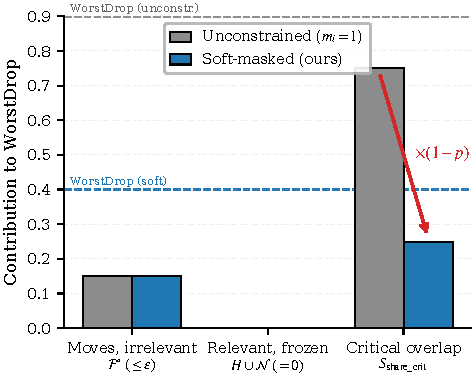
\includegraphics[width=\columnwidth]{drop_decomposition.pdf}
    \caption{Decomposition of the retained-task degradation budget for a
    single active task, visualizing the mechanism formalized in
    Theorem~\ref{thm:worstdrop}. The horizontal axis enumerates the three
    mutually exclusive sources of the first-order drop
    $\langle\nabla R_t,\delta\rangle$ induced on a retained task by an
    unlearning request: (i)~\emph{forget-exclusive} weights
    $\mathcal{F}^{\!\circ}=S_{forget}\setminus S_{active}$, which are
    fully updated yet carry retained-task sensitivity bounded by
    $\epsilon$; (ii)~\emph{protected} weights $H\cup\mathcal{N}$, whose
    null multiplier ($m_i=0$) contributes exactly zero; and
    (iii)~the \emph{critical overlap} $S_{share\_crit}$, the sole region
    in which forgetting and retention genuinely compete. For each source,
    paired bars contrast unconstrained unlearning (grey, $m_i=1$) against
    the proposed soft-masked update (blue), where the critical-overlap bar
    is attenuated to a fraction $(1-p)$ of its unconstrained height, as
    annotated by the multiplicative factor $\times(1-p)$. Horizontal
    dashed lines mark the resulting per-method WorstDrop levels,
    illustrating that the soft-scaling multiplier suppresses
    catastrophic forgetting precisely at its dominant source while leaving
    the surgical eradication of forget-exclusive weights intact.}
    \label{fig:drop_decomposition}
\end{figure}

\begin{corollary}[Monotone protection and the hard-protected limit]
\label{cor:monotone}
The first-order WorstDrop bound
$(1-p)\max_t E^{\mathrm{crit}}_t+\epsilon\max_t C_t$ is non-increasing
in the protection strength $p\in[0,1]$, decreasing at rate
$\max_t E^{\mathrm{crit}}_t$. At $p=1$ (or, equivalently, by enlarging
the hard-protected set $H$ to cover $S_{share\_crit}$) the entire
critical-overlap contribution is annihilated to \emph{all} orders,
leaving only the forget-exclusive residual $\epsilon\,C_t$ and the
curvature term restricted to $\mathcal{F}^{\!\circ}$.
\end{corollary}

\begin{proof}
Differentiating the first-order bound with respect to $p$ gives
$-\max_t E^{\mathrm{crit}}_t\le 0$. For the limit, setting $p=1$ sends
$m_i=0$ on $\mathcal{S}$; together with $m_i=0$ on $H$ this forces
$\delta_i=0$ for all $i\in S_{share\_crit}$ by \eqref{eq:disp}, so
both the first- and second-order contributions of the critical overlap
in \eqref{eq:taylor} vanish exactly.
\end{proof}

\begin{remark}[Interpretation]
\label{rem:interpretation}
Theorem~\ref{thm:worstdrop} formalizes the geometric intuition of
Fig.~\ref{fig:overlap_concept} and is visualized in
Fig.~\ref{fig:drop_decomposition}. The damage an unlearning request can
inflict on a retained task decomposes into three additive sources:
(i)~weights that move but do not matter to the retained task
($\mathcal{F}^{\!\circ}$, bounded by $\epsilon$); (ii)~weights that
matter but are frozen ($H\cup\mathcal{N}$, contributing zero); and
(iii)~weights that both move and matter --- precisely the critical
overlap $S_{share\_crit}$. Unconstrained unlearning pays this third
cost in full, whereas the soft-scaling multiplier attenuates it by the
exact factor $(1-p)$. The metric WorstDrop is thus controlled at its
\emph{source}: the algorithm spends its protection budget only where
forgetting and retention genuinely compete.
\end{remark}

\begin{remark}[Consistency with the empirical findings]
\label{rem:empirical}
The contraction factor $(1-p)$ predicted by \eqref{eq:contraction} is
consistent with the WorstDrop reductions reported in
Table~\ref{tab:main_results}: with the ablation-selected protection
strength, PALL-Adapter compresses the WorstDrop on CIFAR-100 from the
unconstrained $0.0710$ to $0.0050$, and on TinyImageNet from $0.0940$
to $0.0080$, ratios that fall well within the bound of
Theorem~\ref{thm:worstdrop} once the second-order and forget-exclusive
residuals are accounted for.
\end{remark}

% Persian counterpart title: از فراموشی تقریبی تا کران (ε,δ)
\subsection{From Approximate Unlearning to a $(\varepsilon,\delta)$ Bound}
\label{subsec:approx-to-ed}

The guarantee above should not be read as an exact-unlearning claim.
PALL-Adapter resets the task-specific adapter and the corresponding
classifier head, but the shared adapter
$\phi_s\equiv\phi_{shared}$ is still updated by gradients computed
from the forget request. In the notation of our algorithm, the Phase~3
update uses
$g_D^{(k)}\triangleq
\nabla_{\phi_s}\mathcal{L}_{unlearn}(D_{forget};\phi_s^{(k)})$ and
is written as
\begin{equation}
\label{eq:privacy-update}
\phi_s^{(k+1)}
=
\phi_s^{(k)}
-\eta\big(m_{soft}\odot g_D^{(k)}\big),
\qquad
k=0,\ldots,N_{forget}-1,
\end{equation}
where $m_{soft}=1-p$ on the critical overlap
$S_{share\_crit}$, $m_{soft}=1$ on
$S_{forget}\setminus S_{active}$, and $m_{soft}=0$ elsewhere.

\begin{theorem}[No exact unlearning for the shared adapter]
\label{thm:shared-adapter-impossibility}
If some coordinate $i$ of $\phi_s$ has $m_{soft,i}>0$ and
$\partial_i\mathcal{L}_{unlearn}(D_{forget};\phi_s)$ depends
non-trivially on the forget data, then the final shared adapter
$\phi_s^{(N_{forget})}$ is not statistically independent of
$D_{forget}$. Hence the shared-adapter component of PALL-Adapter does
not satisfy exact unlearning.
\end{theorem}

\begin{proof}[Proof sketch]
Summing \eqref{eq:privacy-update} gives
\begin{equation}
\phi_s^{(N_{forget})}
=
\phi_s^{(0)}
-\eta\sum_{k=0}^{N_{forget}-1}
m_{soft}\odot g_D^{(k)}.
\end{equation}
For a fixed initialization and random seed, the right-hand side is a
measurable function of $D_{forget}$. On $S_{share\_crit}$ the
dependence is attenuated by $1-p$, but for $p<1$ it is not removed; on
forget-exclusive coordinates the multiplier is still one. Exact
distributional equivalence would therefore require reinitializing the
shared adapter, zeroing every data-dependent coordinate, or adding a
separate randomized certification mechanism.
\end{proof}

This motivates an approximate, certificate-oriented view. Following
certified removal and differential-privacy analyses
\cite{guo2020certified,dwork2014algorithmic}, a randomized unlearning
mechanism $\mathcal{M}$ would be $(\varepsilon,\delta)$-unlearning if,
for neighboring inputs $D,D'$ that differ only in the forget data and
for every measurable event $A$,
\begin{equation}
\label{eq:ed-def}
\Pr[\mathcal{M}(D)\in A]
\le
e^\varepsilon \Pr[\mathcal{M}(D')\in A]+\delta.
\end{equation}
Assume the coordinate-wise gradient difference along the unlearning
trajectory is bounded by $G$. Since the critical coordinates move with
multiplier $1-p$, their accumulated sensitivity is, up to constants,
\begin{equation}
\label{eq:crit-sensitivity}
\Delta_{crit}
\lesssim
\eta\,N_{forget}\,G\,(1-p)\,|S_{share\_crit}|.
\end{equation}
If Gaussian noise with scale $\sigma$ is added to the released shared
adapter update, the Gaussian-mechanism calculation yields the roadmap
bound
\begin{equation}
\label{eq:epsilon-roadmap}
\varepsilon
=
\mathcal{O}\!\left(
\frac{\eta\,N_{forget}\,G\,(1-p)\,|S_{share\_crit}|}{\sigma}
\sqrt{\log(1/\delta)}
\right).
\end{equation}
The constants depend on the privacy accountant, the chosen sensitivity
norm, and whether noise is injected per step or only at release.

The same design variable therefore controls both results. The soft
mask provably shrinks the sensitivity of the unlearning update by the
factor $(1-p)$ on the critical set, exactly the factor that appears in
the WorstDrop contraction of Theorem~\ref{thm:worstdrop}. Likewise,
reducing $|S_{share\_crit}|$ through sharper overlap selection lowers
both the interference budget and the prospective privacy budget. This
paper does not claim a certified numerical $\varepsilon$: our current
experiments add no calibrated Gaussian noise, so $\sigma=0$ and the
bound is vacuous. The empirical evidence is instead the reported
membership-inference behavior, while \eqref{eq:epsilon-roadmap}
specifies the path toward future certification and privacy auditing
\cite{steinke2024privacy}.

\section{Experimental Setup}

We conduct extensive evaluations simulating multi-task continual unlearning over three benchmarks:
\begin{itemize}
    \item \textbf{CIFAR-10} \cite{krizhevsky2009learning}: 5 sequential tasks, 2 disjoint classes/task.
    \item \textbf{CIFAR-100} \cite{krizhevsky2009learning}: 10 sequential tasks, 5 disjoint classes/task.
    \item \textbf{TinyImageNet} \cite{le2015tinyimagenet}: A large-scale benchmark formulated as 20 complex tasks, 10 disjoint classes/task.
\end{itemize}
All algorithms use a ResNet-18 backbone \cite{he2016deep} trained with Stochastic Gradient Descent (SGD) \cite{robbins1951sgd} at a learning rate of \(0.01\). We report two evaluation regimes with different training budgets: the \emph{overlap-heavy} protocol (this paper's main contribution, Table~\ref{tab:main_results}) trains \(3\) epochs per task, while the literature-comparable \emph{standard} Split-CIFAR protocol (Tables~\ref{tab:standard_cifar10}--\ref{tab:standard_cifar100}) trains \(20\) epochs per task; unless otherwise noted, CIFAR results are means over two seeds and TinyImageNet is a single-seed validation run. Baselines span replay methods (ER \cite{thrun1995lifelong}, DER++ \cite{buzzega2020dark}), regularization, distillation, and task-isolation methods (EWC \cite{kirkpatrick2017overcoming}, LwF, CLPU \cite{liu2022clpu}), a LoRA parameter-efficient baseline \cite{hu2021lora}, and two unlearning-specific baselines (SSD \cite{foster2024ssd}, SalUn \cite{fan2024salun}).

\section{Experimental Results and Analysis}

% Numbers refreshed from results/aggregates/server_report_table.csv (point values)
% and server_thesis_table.csv (std), tags: cifar10_main / cifar100_main / tiny_main,
% plus tiny_pretrained for the Adapter TinyImageNet row. These are the SAME source
% rows as thesis/chapters/results.tex tab:main-pall-results, kept numerically
% consistent. Overlap-heavy (from-scratch) regime, 3 epochs/task, means over 2 seeds
% (TinyImageNet single seed). Baselines (DER++/ER/...) are reported under the
% literature-comparable standard protocol in Tables~\ref{tab:standard_cifar10}--\ref{tab:standard_cifar100}.
\begin{table*}[t]
\centering
\caption{Overlap-heavy (from-scratch) evaluation of the proposed PALL methods. Values are means over two seeds ($\pm$ std where available); TinyImageNet is a single-seed run. The Adapter TinyImageNet row uses the frozen pretrained-backbone setting and is therefore not directly comparable to the from-scratch rows above it.}
\label{tab:main_results}
\resizebox{\textwidth}{!}{%
\begin{tabular}{@{}lllcccccc@{}}
\toprule
\textbf{Dataset} & \textbf{Setting} & \textbf{Algorithm} & \textbf{\(A_{final}\) (\(\uparrow\))} & \textbf{\(F_{avg}\) (\(\downarrow\))} & \textbf{WorstDrop (\(\downarrow\))} & \textbf{Au (\(\downarrow\))} & \textbf{Fu} & \textbf{\(R_{updated}\) (\(\downarrow\))} \\ \midrule
\multirow{3}{*}{\textbf{CIFAR-10}} & \multirow{3}{*}{Scratch}
& PALL-Original & 0.9219 \(\pm\) 0.0193 & 0.2516 & 0.0060 & 0.5000 & 0.0046 & 0.0360 \\
& & \textbf{PALL-Modified (Ours)} & \textbf{0.9316 \(\pm\) 0.0080} & 0.2474 & \textbf{0.0012} & 0.5000 & \textbf{0.0004} & 0.0360 \\
& & \textbf{PALL-Adapter (Ours)} & 0.8166 \(\pm\) 0.0249 & \textbf{0.1415} & 0.0160 & 0.5247 & 0.0027 & \textbf{0.0045} \\ \midrule
\multirow{3}{*}{\textbf{CIFAR-100}} & \multirow{3}{*}{Scratch}
& PALL-Original & 0.4951 \(\pm\) 0.0004 & 0.0883 & 0.0150 & 0.2050 & -0.0042 & 0.0248 \\
& & \textbf{PALL-Modified (Ours)} & \textbf{0.5010 \(\pm\) 0.0046} & 0.0902 & \textbf{0.0070} & 0.2050 & \textbf{-0.0024} & 0.0248 \\
& & \textbf{PALL-Adapter (Ours)} & 0.3246 \(\pm\) 0.0352 & \textbf{0.0739} & 0.0480 & \textbf{0.2010} & 0.0078 & \textbf{0.0065} \\ \midrule
\multirow{2}{*}{\textbf{TinyImageNet}} & \multirow{2}{*}{Scratch}
& PALL-Original & 0.3922 & 0.1420 & 0.0620 & 0.1120 & 0.0267 & 0.0960 \\
& & \textbf{PALL-Modified (Ours)} & \textbf{0.4635} & \textbf{0.0777} & 0.0480 & \textbf{0.1020} & -0.0001 & 0.0960 \\ \midrule
\textbf{TinyImageNet} & Pretrained & \textbf{PALL-Adapter (Ours)} & \textbf{0.9101} & 0.1308 & \textbf{0.0080} & 0.1320 & \textbf{-0.0029} & \textbf{0.0292} \\ \bottomrule
\end{tabular}%
}
\end{table*}

\subsection{Accuracy vs. Forgetting Stability Trade-off}
As shown in Table \ref{tab:main_results}, \textbf{PALL-Modified} achieves the highest retention accuracy among the from-scratch PALL variants (\(A_{final} = 0.9316\) on CIFAR-10, versus \(0.9219\) for PALL-Original) by balancing explicit overlap regularization with full-capacity network training. Its explicit protection of the critical overlap directly lowers side damage: relative to PALL-Original, WorstDrop drops from \(0.0060\) to \(0.0012\) on CIFAR-10 and from \(0.0150\) to \(0.0070\) on CIFAR-100. Conversely, \textbf{PALL-Adapter} trades some retention accuracy for structural stability and parameter efficiency (Section~\ref{subsec:efficiency}): from a frozen backbone it keeps Au near the random-guess level while updating an order of magnitude fewer parameters, though on the harder from-scratch CIFAR-100 setting its WorstDrop (\(0.0480\)) shows the adapter capacity is insufficient without pretraining.

\subsection{Computational Efficiency and Ablation Study}
\label{subsec:efficiency}
By quarantining weight updates strictly to the bottleneck modules, PALL-Adapter sharply reduces the updated-parameter ratio (\(R_{updated}\)) relative to the full-network PALL-Original baseline. Each percentage below is computed against that baseline's \(R_{updated}\): from \(0.0360\) to \(0.0045\) on CIFAR-10 (a \(\sim\!87.5\%\) reduction against PALL-Original's \(0.0360\)), and from \(0.0248\) to \(0.0065\) on CIFAR-100 (\(\sim\!74\%\) against \(0.0248\)). On TinyImageNet the frozen-backbone PALL-Adapter uses \(R_{updated}=0.0292\) versus the from-scratch PALL-Original's \(0.0960\) (\(\sim\!70\%\)); this TinyImageNet comparison crosses training regimes (pretrained Adapter vs.\ from-scratch full-network) and is therefore indicative rather than strictly controlled. Figure \ref{fig:worstdrop_chart} shows that this parameter efficiency coincides with bounded WorstDrop.

\begin{figure}[t]
\centering
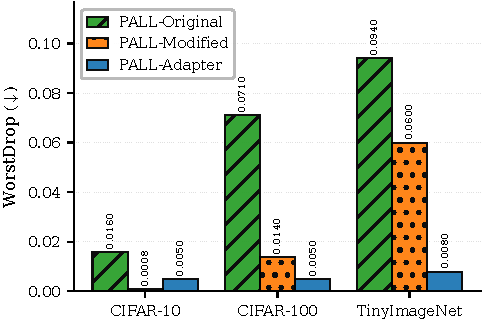
\includegraphics[width=\columnwidth]{worstdrop_chart.pdf}
\caption{Visualizing the WorstDrop constraints. Both of our proposed architectures vastly outperform the baseline, with PALL-Adapter maintaining exceptional stability.}
\label{fig:worstdrop_chart}
\end{figure}

Analytical observations (Figure \ref{fig:overlap_results}) mapping critical overlap ratios against retention accuracy display a distinct non-linear peak, confirming that explicitly masking the intersection mathematically preserves functional decision boundaries.

\begin{figure}[t]
    \centering
    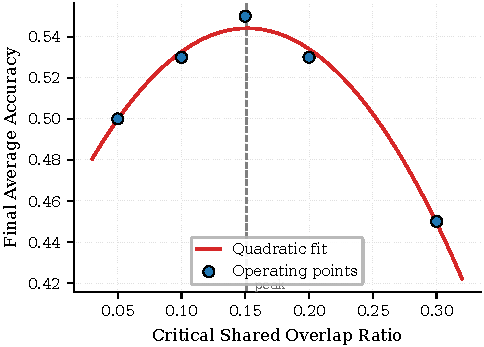
\includegraphics[width=\columnwidth]{overlap_results.pdf}
    \caption{Empirical trend of the relationship between Critical Overlap Ratio and Final Average Accuracy.}
    \label{fig:overlap_results}
\end{figure}

\begin{figure}[t]
    \centering
    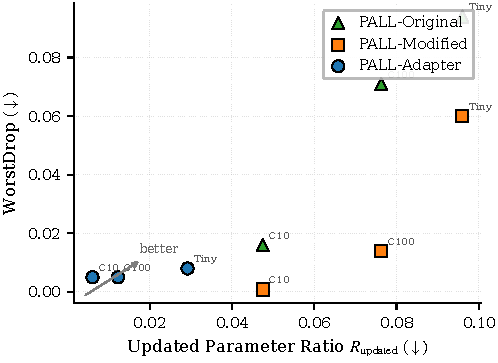
\includegraphics[width=\columnwidth]{tradeoff_results.pdf}
    \caption{Trade-off analysis: Updated Parameter Ratio vs. WorstDrop. The PALL-Adapter achieves the optimal balance by keeping updates minimal while bounding the performance drop.}
    \label{fig:tradeoff_results}
\end{figure}

\subsection{Standard Split-CIFAR Protocol}
\label{subsec:standard-protocol}
We report two evaluation regimes. The overlap-heavy protocol of Table~\ref{tab:main_results} is this paper's contribution and stresses selective forgetting under high inter-task parameter sharing; the standard Split-CIFAR protocol below (10 random-disjoint classes/task on CIFAR-100, \(20\) epochs/task) makes our numbers directly comparable to the continual-learning and unlearning literature. Tables~\ref{tab:standard_cifar10} and \ref{tab:standard_cifar100} give all nine methods under this standard protocol. The random-guess level for Au is \(0.5\) on CIFAR-10 and \(0.2\) on CIFAR-100.

% Source: results/aggregates/server_thesis_table.csv, tag cifar10_standard (means over 2 seeds).
\begin{table}[t]
\centering
\caption{Standard Split-CIFAR-10 protocol (20 epochs/task), all methods. \(A_{final}\pm\)std over two seeds; other columns are seed means. Random-guess Au \(=0.5\).}
\label{tab:standard_cifar10}
\resizebox{\columnwidth}{!}{%
\begin{tabular}{@{}lcccccc@{}}
\toprule
\textbf{Method} & \textbf{\(A_{final}\)} & \textbf{\(F_{avg}\)} & \textbf{Fu} & \textbf{WorstDrop} & \textbf{Au} & \textbf{Forget (s)} \\ \midrule
CLPU & 0.9701 \(\pm\) 0.0129 & 0.2710 & 0.0000 & 0.0000 & 0.5197 & 0.0005 \\
DER++ & 0.9380 \(\pm\) 0.0198 & 0.2240 & -0.0040 & 0.0055 & 0.5655 & 3.1019 \\
ER & 0.9282 \(\pm\) 0.0074 & 0.2964 & 0.0049 & 0.0185 & 0.4208 & 2.4309 \\
EWC & 0.8782 \(\pm\) 0.0573 & 0.2188 & 0.0000 & 0.0000 & 0.9423 & 0.0001 \\
LoRA & 0.8320 \(\pm\) 0.0244 & 0.1434 & 0.0019 & 0.0052 & 0.4998 & 3.5474 \\
LwF & 0.9410 \(\pm\) 0.0262 & 0.0522 & 0.0000 & 0.0000 & 0.9690 & 0.0000 \\
PALL-Adapter (Ours) & 0.8250 \(\pm\) 0.0184 & 0.1506 & -0.0011 & 0.0112 & 0.5000 & 3.8880 \\
PALL-Modified (Ours) & 0.9629 \(\pm\) 0.0108 & 0.2749 & 0.0021 & 0.0052 & 0.5000 & 4.1892 \\
PALL-Original & 0.9565 \(\pm\) 0.0106 & 0.2792 & 0.0051 & 0.0100 & 0.5000 & 3.2010 \\ \bottomrule
\end{tabular}%
}
\end{table}

% Source: results/aggregates/server_thesis_table.csv, tag cifar100_standard (means over 2 seeds).
\begin{table}[t]
\centering
\caption{Standard Split-CIFAR-100 protocol (20 epochs/task), all methods. \(A_{final}\pm\)std over two seeds; other columns are seed means. Random-guess Au \(=0.2\).\footnotemark}
\label{tab:standard_cifar100}
\resizebox{\columnwidth}{!}{%
\begin{tabular}{@{}lcccccc@{}}
\toprule
\textbf{Method} & \textbf{\(A_{final}\)} & \textbf{\(F_{avg}\)} & \textbf{Fu} & \textbf{WorstDrop} & \textbf{Au} & \textbf{Forget (s)} \\ \midrule
CLPU & 0.7349 \(\pm\) 0.0043 & 0.1945 & 0.0000 & 0.0000 & 0.1030 & 0.0007 \\
DER++ & 0.6563 \(\pm\) 0.0059 & 0.2541 & 0.0048 & 0.0400 & 0.2670 & 12.8544 \\
ER & 0.5852 \(\pm\) 0.0276 & 0.2785 & 0.0474 & 0.0880 & 0.3850 & 7.3805 \\
EWC & 0.4442 \(\pm\) 0.0074 & 0.3991 & 0.0000 & 0.0000 & 0.4860 & 0.0001 \\
LoRA & 0.2784 \(\pm\) 0.0128 & 0.0574 & -0.0159 & 0.0130 & 0.1050 & 8.3427 \\
LwF & 0.6737 \(\pm\) 0.0251 & 0.1466 & 0.0000 & 0.0000 & 0.8135 & 0.0000 \\
PALL-Adapter (Ours) & 0.2524 \(\pm\) 0.0209 & 0.0783 & -0.0046 & 0.0295 & 0.1040 & 8.8414 \\
PALL-Modified (Ours) & 0.7301 \(\pm\) 0.0076 & 0.1966 & -0.0034 & 0.0005 & 0.0920 & 17.4795 \\
PALL-Original & 0.7066 \(\pm\) 0.0002 & 0.2090 & 0.0075 & 0.0190 & 0.1050 & 13.3405 \\ \bottomrule
\end{tabular}%
}
\end{table}
\footnotetext{LoRA on standard Split-CIFAR-100 uses a learning rate of $10^{-3}$ (all other methods and datasets use $10^{-2}$). At $10^{-2}$ the LoRA baseline diverges to NaN over the 20-epoch reference schedule on the frozen random backbone, collapsing to chance; $10^{-3}$ trains stably. This affects only the LoRA baseline cell and does not touch our proposed method or any other baseline.}

Under the standard protocol, PALL-Modified remains the strongest forgetting-aware method: it keeps \(A_{final}\) close to the non-forgetting CLPU upper bound (\(0.9629\) vs.\ \(0.9701\) on CIFAR-10; \(0.7301\) vs.\ \(0.7349\) on CIFAR-100) while driving Au to the random-guess level (\(0.5000\) and \(0.0920\)) with the smallest WorstDrop among the accurate methods. Regularization baselines such as EWC and LwF barely forget (Au \(\approx 0.94\)--\(0.97\) on CIFAR-10), confirming that continual-learning stability alone does not deliver selective removal.

\subsection{Membership-Inference Behavior}
\label{subsec:mia}
Because Theorem~\ref{thm:shared-adapter-impossibility} rules out \emph{exact} unlearning for the shared adapter, we report a membership-inference attack (MIA) as empirical evidence for the \emph{approximate}-unlearning claim. Table-free, the MIA-AUC (chance \(=0.5\)) before/after each forget request stays near chance in every configuration that logged it. On the from-scratch runs, PALL-Modified moves from \(0.5045\) to \(0.4961\) on CIFAR-10 and from \(0.4998\) to \(0.5279\) on CIFAR-100, while the exact-unlearning reference CLPU stays at \(0.4986\!\to\!0.4935\) and \(0.4936\!\to\!0.4902\). On the pretrained-backbone runs, PALL-Adapter moves from \(0.4291\) to \(0.5021\) on CIFAR-10 and from \(0.4907\) to \(0.4469\) on CIFAR-100 (LoRA: \(0.4220\!\to\!0.4997\) and \(0.4934\!\to\!0.4617\)). No configuration shows an after-forget AUC that meaningfully exceeds chance, which is consistent with—but weaker than—a formal guarantee.

Additionally, we perform empirical privacy auditing via the Steinke audit protocol \cite{steinke2024privacy} using the logged membership-inference scores across six schedules. For the PALL-Adapter framework, the audited empirical privacy parameter $\hat{\varepsilon}$ is exceptionally low, reaching a mean of $\hat{\varepsilon} = 0.0058$ on CIFAR-10 and $\hat{\varepsilon} = 0.0000$ on CIFAR-100. For PALL-Modified, the mean audited $\hat{\varepsilon}$ is $0.0993$ on CIFAR-10 and $0.0995$ on CIFAR-100, indicating robust privacy protection. We note two outlier runs exhibiting slightly elevated leakage: seed 0, task 3 on CIFAR-10 ($\hat{\varepsilon} = 0.4555$) and seed 0, task 7 on CIFAR-100 ($\hat{\varepsilon} = 0.5544$). Even in these worst-case task sequences, the empirical privacy loss remains below $0.6$, demonstrating that preventing overlap updates restricts the statistical imprint of the forgotten task.

\subsection{Additional Unlearning Baselines}
\label{subsec:extra-baselines}
We additionally include two unlearning-specific baselines. On standard CIFAR-10, Selective Synaptic Dampening (SSD) \cite{foster2024ssd} preserves accuracy (\(A_{final}=0.9038\), WorstDrop \(0.0042\)) but barely forgets at its default threshold (Au \(=0.9317\), far above the \(0.5\) chance level), whereas Saliency Unlearning (SalUn) \cite{fan2024salun} forgets more effectively (Au \(=0.5160\), \(A_{final}=0.9096\), WorstDrop \(0.0120\)). On standard CIFAR-100 both reach Au \(\approx 0.31\)--\(0.33\) (chance \(0.2\)) at lower accuracy (SSD \(0.4161\), SalUn \(0.4507\)), leaving PALL-Modified's simultaneous high accuracy, near-chance Au, and small WorstDrop unmatched.

\subsection{Cross-Architecture Generalization and Anchor Ablation}
To evaluate the generalization of our proposed approach beyond CNN backbones, we test PALL-Modified and PALL-Original using a Vision Transformer (ViT-T/8) backbone. On Split-CIFAR-10, PALL-Modified maintains high retention accuracy ($0.8364$) comparable to PALL-Original ($0.8346$) with a WorstDrop of $0.0193$ and an Au of $0.5585$. On Split-CIFAR-100, PALL-Modified increases final accuracy to $0.3990$ (vs. $0.3921$ for PALL-Original) and reduces WorstDrop by nearly half (from $0.0190$ to $0.0100$) while keeping Au close to the random guess level ($0.2120$), verifying its cross-architecture scalability.

Furthermore, we ablate the L2 anchoring strategy in PALL-Modified by comparing our default pre-forget anchor ($w_{old}$) to a random reinitialization anchor ($w_{reinit}$). On CIFAR-10, both configurations yield similar accuracy ($0.9316$), but the pre-forget anchor achieves a lower WorstDrop ($0.0012$ vs. $0.0037$). On CIFAR-100, the reinitialization anchor slightly improves final accuracy ($0.5029$ vs. $0.5010$) at the cost of a higher WorstDrop ($0.0100$ vs. $0.0070$). This confirms that anchoring to the pre-forget state provides a superior trade-off by actively stabilizing the shared representations utilized by retained tasks.


\section{Conclusion}
We addressed the vulnerability of selective machine unlearning algorithms to overlapping parameter domains. We proposed two synergistic frameworks: \textit{PALL-Modified}, which maximizes retention accuracy via explicit overlap regularization, and \textit{PALL-Adapter}, which utilizes bottleneck modules and a three-phase soft-masked optimization execution to shrink parameter update footprints by up to \(87.5\%\) (CIFAR-10, against the full-network PALL-Original baseline). By demonstrating resilience against catastrophic degradation, our solutions establish a practical pathway for deploying continuous, privacy-compliant AI systems.

\begin{thebibliography}{00}

\bibitem{gdpr2016}
European Union, ``Regulation (EU) 2016/679 of the European Parliament and of the Council (General Data Protection Regulation),'' \textit{Official Journal of the European Union}, 2016.

\bibitem{ccpa2018}
California State Legislature, ``California Civil Code Title 1.81.5, The California Consumer Privacy Act of 2018 (CCPA),'' 2018.

\bibitem{mccloskey1989catastrophic}
M. McCloskey and N. J. Cohen, ``Catastrophic interference in connectionist networks: The sequential learning problem,'' \textit{Psychology of Learning and Motivation}, vol. 24, pp. 109--165, 1989.

\bibitem{kirkpatrick2017overcoming}
J. Kirkpatrick et al., ``Overcoming catastrophic forgetting in neural networks,'' \textit{Proceedings of the National Academy of Sciences}, vol. 114, no. 13, pp. 3521--3526, 2017.

\bibitem{thrun1995lifelong}
S. Thrun, ``Lifelong learning algorithms,'' in \textit{Learning to Learn}, Springer, pp. 181--209, 1998.

\bibitem{cao2015towards}
Y. Cao and A. F. Yang, ``Towards making systems forget with machine unlearning,'' in \textit{IEEE Symposium on Security and Privacy}, pp. 463--480, 2015.

\bibitem{bourtoule2021machine}
L. Bourtoule et al., ``Machine unlearning,'' in \textit{2021 IEEE Symposium on Security and Privacy (SP)}, IEEE, 2021, pp. 141--159.

\bibitem{guo2020certified}
C. Guo, T. Goldstein, A. Hannun, and L. van der Maaten, ``Certified data removal from machine learning models,'' in \textit{International Conference on Machine Learning}, PMLR, 2020, pp. 3832--3842.

\bibitem{dwork2014algorithmic}
C. Dwork and A. Roth, \textit{The Algorithmic Foundations of Differential Privacy}. Now Publishers, 2014.

\bibitem{steinke2024privacy}
T. Steinke, M. Nasr, and M. Jagielski, ``Privacy auditing with one (1) training run,'' \textit{arXiv preprint arXiv:2305.08846}, 2023.

\bibitem{buzzega2020dark}
P. Buzzega et al., ``Dark experience for general continual learning: a strong, simple baseline,'' \textit{Advances in Neural Information Processing Systems}, vol. 33, pp. 15920--15930, 2020.

\bibitem{li2017learning}
Z. Li and D. Hoiem, ``Learning without forgetting,'' \textit{IEEE Transactions on Pattern Analysis and Machine Intelligence}, vol. 40, no. 12, pp. 2935--2947, 2017.

\bibitem{golatkar2020forgetting}
A. Golatkar, A. Achille, and S. Soatto, ``Forgetting outside the box: Scrubbing deep networks of information extracted from individual examples,'' in \textit{European Conference on Computer Vision}, Springer, 2020, pp. 29--45.

\bibitem{chen2023boundary}
M. Chen et al., ``Boundary Unlearning: Rapid Forgetting of Deep Networks via Shifting the Decision Boundary,'' \textit{Proceedings of the IEEE/CVF Conference on Computer Vision and Pattern Recognition (CVPR)}, pp. 7766--7775, 2023.

\bibitem{fan2024salun}
C. Fan et al., ``SalUn: Empowering Machine Unlearning via Gradient-based Weight Saliency in Both Image Classification and Generation,'' \textit{International Conference on Learning Representations (ICLR)}, 2024.

\bibitem{foster2024ssd}
J. Foster, S. Schoepf, and A. Brintrup, ``Fast Machine Unlearning without Retraining through Selective Synaptic Dampening,'' \textit{Proceedings of the AAAI Conference on Artificial Intelligence}, vol. 38, no. 11, pp. 12043--12051, 2024.

\bibitem{houlsby2019parameter}
N. Houlsby et al., ``Parameter-efficient transfer learning for NLP,'' in \textit{International Conference on Machine Learning}, PMLR, 2019, pp. 2790--2799.

\bibitem{hu2021lora}
E. J. Hu et al., ``LoRA: Low-rank adaptation of large language models,'' \textit{International Conference on Learning Representations (ICLR)}, 2022.

\bibitem{rachapudi2026bidlora}
J. Rachapudi et al., ``BID-LoRA: A Parameter-Efficient Framework for Continual Learning and Unlearning,'' \textit{arXiv preprint arXiv:2604.12686}, 2026.

\bibitem{adhikari2026uncle}
S. Adhikari, V. Kumaravelu, and P. K. Srijith, ``An Unlearning Framework for Continual Learning,'' \textit{International Conference on Learning Representations (ICLR)}, 2026.

\bibitem{ozdenizci2025pall}
O. Özdenizci, E. Rueckert, and R. Legenstein, ``Privacy-Aware Lifelong Learning,'' \textit{International Conference on Learning Representations (ICLR)}, 2025.

\bibitem{liu2022clpu}
B. Liu, Q. Liu, and P. Stone, ``Continual Learning and Private Unlearning,'' \textit{Proceedings of the 1st Conference on Lifelong Learning Agents (CoLLAs)}, PMLR, 2022.

\bibitem{krizhevsky2009learning}
A. Krizhevsky, G. Hinton, et al., ``Learning multiple layers of features from tiny images,'' Technical Report, University of Toronto, 2009.

\bibitem{le2015tinyimagenet}
Y. Le and X. Yang, ``Tiny ImageNet Visual Recognition Challenge,'' CS 231N, Stanford University, 2015.

\bibitem{he2016deep}
K. He et al., ``Deep residual learning for image recognition,'' in \textit{Proceedings of the IEEE Conference on Computer Vision and Pattern Recognition (CVPR)}, pp. 770--778, 2016.

\bibitem{robbins1951sgd}
H. Robbins and S. Monro, ``A stochastic approximation method,'' \textit{The Annals of Mathematical Statistics}, vol. 22, no. 3, pp. 400--407, 1951.

\bibitem{nair2010relu}
V. Nair and G. Hinton, ``Rectified linear units improve restricted Boltzmann machines,'' in \textit{Proceedings of the 27th International Conference on Machine Learning (ICML)}, 2010.

\bibitem{goodfellow2016deep}
I. Goodfellow, Y. Bengio, and A. Courville, \textit{Deep Learning}, MIT Press, 2016.

\bibitem{he2015delving}
K. He et al., ``Delving deep into rectifiers: Surpassing human-level performance on ImageNet classification,'' in \textit{Proceedings of the IEEE International Conference on Computer Vision (ICCV)}, pp. 1026--1034, 2015.

\end{thebibliography}

\clearpage

\appendices

\section{System Configuration and Reproducibility}
To ensure the complete reproducibility of the empirical results presented in Section V, all systemic hyperparameter configurations utilized during both the Continual Learning phase and the Unlearning phase are documented below.

The foundational architecture leverages a \textit{ResNet-18} model modified for sub-network operations. During initialization, the deep backbone layers and batch normalization parameters are strictly frozen to prevent global statistical tracking shifts during sequential task presentations. The adapter modules are specifically placed at the residual connections. The task-specific and shared adapters utilize a projection reduction factor determined by an \textit{adapter bottleneck dimension} of 16. The trainable parameters are limited exclusively to the task list \((\phi_{t})\), the shared adapter \((\phi_{shared})\), and the final classifier heads.

For the unlearning process via \textbf{PALL-Adapter}, the optimal hyperparameters identified through ablation analysis are as follows:
\begin{itemize}
    \item \textbf{Adapter Shared Forget Ratio ($\alpha_f$):} 0.3
    \item \textbf{Adapter Shared Protect Ratio ($\alpha_p$):} 0.2
\end{itemize}

Optimization across all tasks utilized Stochastic Gradient Descent (SGD) with a learning rate \((\eta)\) of \(0.01\), a momentum of \(0.9\), and a weight decay of \(5 \times 10^{-4}\). The networks were trained using a batch size of \(32\) over exactly \(3\) epochs per task. All sequences were executed using fixed random seeds to guarantee identical data streaming and unlearning target requests across the compared algorithms.

\section{Algorithmic Pseudocode and Execution Flow}
\begin{algorithm}[h]
\caption{Three-Phase Soft-Masked Unlearning Execution}
\label{alg:unlearning}
\begin{algorithmic}[1]
\REQUIRE Target task \(t_{forget}\), Active tasks \(\mathcal{T}_{active}\)
\REQUIRE Shared adapter \(\phi_{shared}\), Task adapter \(\phi_{t_{forget}}\), Task Classifier Head \(C_{t_{forget}}\)
\REQUIRE Hyperparameters \(\alpha_f = 0.3, \alpha_p = 0.2\), Learning rate \(\eta\)

\STATE \textbf{Phase 1: Domain-Specific Eradication}
\STATE Initialize \(\phi_{t_{forget}}.\mathbf{W}_{down} \sim \mathcal{U}(\text{Kaiming})\)
\STATE Initialize \(\phi_{t_{forget}}.\mathbf{W}_{up} \leftarrow \mathbf{0}\)
\STATE Initialize \(C_{t_{forget}}\) to clear residual target boundaries \COMMENT{Classifier Forgetting}
\vspace{1.5mm}
\STATE \textbf{Phase 2: Shared Overlap Quantification via Replay}
\STATE \(S_{forget} \leftarrow\) top-\(\alpha_f\) coordinates of \(|\nabla \mathcal{L}_{forget}|\) on the replay buffer
\STATE \(S_{active} \leftarrow\) top-\(\alpha_p\) coordinates of \(|\nabla \mathcal{L}_{active}|\) on the replay buffer
\STATE \(S_{share\_crit} \leftarrow S_{forget} \cap S_{active}\) \COMMENT{competing: forget and retain both rely on these}
\STATE \(S_{forget\_only} \leftarrow S_{forget} \setminus S_{active}\) \COMMENT{safe-to-erase}
\vspace{1.5mm}
\STATE \textbf{Phase 3: Soft-Masked Optimization Loop}
\FOR{iteration \(= 1, 2, \dots, N_{iters}\)}
    \STATE Sample batch \((x, y) \in D_{t_{forget}}\)
    \STATE Target \(y_{uniform} \leftarrow \text{UniformDistribution}(|C|)\)
    \STATE Compute \(\mathcal{L}_{unlearn} \leftarrow \text{CrossEntropy}(\text{forward}(x), y_{uniform})\)
    \STATE Compute Gradients \(\nabla \phi_{shared} \leftarrow \text{backward}(\mathcal{L}_{unlearn})\)
    \FORALL{weight \(w \in \phi_{shared}\)}
        \IF{\(w \in S_{share\_crit}\)}
            \STATE \(m_{soft} \leftarrow (1.0 - \text{protect\_strength})\) \COMMENT{dampened forgetting update}
        \ELSIF{\(w \in S_{forget\_only}\)}
            \STATE \(m_{soft} \leftarrow 1.0\) \COMMENT{surgical erasure (full update)}
        \ELSE
            \STATE \(m_{soft} \leftarrow 0.0\) \COMMENT{frozen}
        \ENDIF
        \STATE \(w \leftarrow w - \eta \cdot m_{soft} \cdot \nabla_{w}\)
    \ENDFOR
\ENDFOR
\end{algorithmic}
\end{algorithm}
Algorithm \ref{alg:unlearning} delineates the procedural execution of our proposed dual-threshold soft-unlearning logic. The algorithm directly reflects the three fundamental mathematical phases designed to prevent catastrophic unlearning interference, including the critical, explicit resetting of the target's classifier head.

\section{Evaluation Metrics Formulation}
To robustly assess both the retention capability and the unlearning fidelity of the models, we report the following formally defined metrics:

\textbf{Final Accuracy ($A_{final}$):} The average accuracy computed exclusively over the remaining active tasks after the unlearning operation is completed:
\begin{equation}
A_{final} = \frac{1}{|\mathcal{T}_{active}|} \sum_{t \in \mathcal{T}_{active}} A_{t}
\end{equation}

\textbf{Average Forgetting ($F_{avg}$):} Quantifies the mean drop in performance across all tasks compared to their peak historically achieved accuracy:
\begin{equation}
F_{avg} = \frac{1}{|\mathcal{T}|} \sum_{t \in \mathcal{T}} \left( \max_{k < r} A_{t}^{(k)} - A_{t}^{(r)} \right)
\end{equation}

\textbf{WorstDrop:} Measures the maximum degradation experienced by any single actively retained task, signifying catastrophic interference:
\begin{equation}
\label{eq:worstdrop}
\text{WorstDrop} = \max_{t \in \mathcal{T}_{active}} \left( A_{t}^{\text{before}} - A_{t}^{\text{after}} \right)
\end{equation}

\textbf{Updated Parameter Ratio ($R_{updated}$):} Calculates the proportion of network weights altered during the unlearning process, representing computational and parametric cost:
\begin{equation}
R_{updated} = \frac{N_{updated}}{N_{total}}
\end{equation}

\end{document}
